% Appendix material owned by writer 3 (extended tables, constants, derivations moved out of the main report)

\subsection{Style-profile schema and per-writer values}

This part of the appendix supports Section~\ref{sec:styleprofile}.
Table~\ref{tab:sty-schema} lists every key of a style-profile file with its meaning and an example value from the profile of writer 153, and Table~\ref{tab:sty-writers} lists the scalar values of all ten stored profiles.

{
\fontsize{9.5}{11.5}\selectfont
\setlength{\tabcolsep}{4pt}
\begin{longtable}{|p{3.2cm}|p{1.6cm}|p{6.6cm}|p{2.5cm}|}
\hline
\textbf{Key} & \textbf{Type} & \textbf{Meaning} & \textbf{Example (153)} \\
\hline
\endfirsthead
\hline
\textbf{Key} & \textbf{Type} & \textbf{Meaning} & \textbf{Example (153)} \\
\hline
\endhead
\hline
\endfoot
\texttt{authorId} & string & Writer identifier. & \texttt{"153"} \\
\hline
\texttt{slantDeg} & float & Median slant of the lines, forward lean positive (Equation~\ref{eq:sty-slant}). & 30.0 \\
\hline
\texttt{xHeightPx} & float & Median pixel x-height of the kept lines. & 33.0 \\
\hline
\texttt{strokeWidthXh} & float & Ink area divided by skeleton length, in x-heights. & 0.189 \\
\hline
\texttt{ascender}, \texttt{descender} & float & Typical reach of tall and descending lower-case glyphs, in x-heights (defaults 1.7 and $-0.6$ if no glyph qualifies). & 1.59, $-1.11$ \\
\hline
\texttt{wordSpaceXh} & float & Word gap measured on the real ink, in x-heights. & 1.59 \\
\hline
\texttt{connectedness} & float & Fraction of adjacent in-word letter pairs that the pen joins (Equation~\ref{eq:sty-conn}). & 0.97 \\
\hline
\texttt{letterAdvance} & dict & Median advance of each character, in x-heights (45 keys). & \texttt{T}: 1.438, \texttt{e}: 1.143 \\
\hline
\texttt{nLines} & int & Number of lines that survived the alignment-confidence cut. & 66 \\
\hline
\texttt{slantMeasRef}, \texttt{ascMeasRef}, \texttt{descMeasRef} & float & Slant (degrees) and ascender and descender reach of the real full lines, measured with the estimators later used on synthesised renders; input of the style calibration (Equation~\ref{eq:syn-cal}). & 30.0, 1.933, $-1.468$ \\
\hline
\texttt{inkFracRef}, \texttt{aspectRef}, \texttt{paperLevel}, \texttt{inkLevel}, \texttt{midFracRef} & float & Ink fraction, width-to-height ratio and grey statistics of the real lines; stored but ignored while the constant pen width is used for rendering. & 0.0620, 14.95, 246, 81, 0.038 \\
\hline
\texttt{glyphs} & dict & Variant library: for each character a list of at most 13 variant dictionaries (38 characters and 280 variants for writer 153). & see below \\
\hline
\texttt{idealGlyphs} & dict & Per-stroke median prototype of a letter (21 characters), with the keys \texttt{strokes}, \texttt{priorD}, \texttt{advance}, \texttt{lead}, \texttt{width}, \texttt{top}, \texttt{bot}, \texttt{entryY}, \texttt{exitY}, \texttt{nPool}. & --- \\
\hline
\texttt{idealMedoid} & dict & The real variant that is most typical of the writer (28 characters), same keys; this is the anchor used by the synthesiser. & --- \\
\hline
\texttt{legibilityLambda} & float & Legibility parameter $\lambda$ of Equations~\ref{eq:syn-global} and~\ref{eq:syn-swap}; added after the build. & 0.45 \\
\hline
\multicolumn{4}{|l|}{\textbf{Keys of one variant in \texttt{glyphs[c][i]}}} \\
\hline
\texttt{char} & string & The character. & \texttt{"e"} \\
\hline
\texttt{strokes} & list & Strokes, each a list of $[x,y]$ points in x-height units, baseline $y=0$, upright. & 2 and 38 points \\
\hline
\texttt{width}, \texttt{advance}, \texttt{lead} & float & Ink width, cell width and gap before the ink, in x-heights. & 0.878, 1.061, 0.0 \\
\hline
\texttt{top}, \texttt{bot} & float & Highest and lowest point. & 0.879, 0.061 \\
\hline
\texttt{entryX}, \texttt{entryY}, \texttt{exitX}, \texttt{exitY} & float & Entry and exit points of the pen for connectors. & $-0.204$, 0.333, 0.767, 0.182 \\
\hline
\texttt{connL}, \texttt{connR} & bool & The pen was joined to the left or right neighbour. & true, true \\
\hline
\texttt{priorD} & float & Cosine distance to the cross-writer letter prior (Equation~\ref{eq:sty-prior}). & 0.1127 \\
\hline
\texttt{denoised} & bool & Present and true if the variant is the denoised prototype. & --- \\
\hline
\caption{Keys of a style-profile file (JavaScript Object Notation).}
\label{tab:sty-schema}
\end{longtable}
}

\begin{table}[h]
\centering
\fontsize{9}{11}\selectfont
\setlength{\tabcolsep}{3pt}
\begin{tabular}{|l|r|r|r|r|r|r|r|r|r|r|r|}
\hline
\textbf{Writer} & \textbf{Lines} & \textbf{Slant ($^\circ$)} & \textbf{$x_h$ (px)} & \textbf{Stroke width} & \textbf{$A$} & \textbf{$D$} & \textbf{Gap} & \textbf{Conn.} & \textbf{$\lambda$} & \textbf{Chars} & \textbf{Var.} \\
\hline
150 & 61 & $-4.5$ & 46 & 0.097 & 1.58 & $-0.72$ & 1.33 & 0.347 & 0.90 & 40 & 295 \\
151 & 58 & 33.0 & 22 & 0.271 & 2.68 & $-1.09$ & 1.59 & 0.981 & 1.00 & 44 & 285 \\
152 & 59 & 19.5 & 46 & 0.103 & 1.48 & $-0.82$ & 1.47 & 0.735 & 0.45 & 37 & 271 \\
153 & 66 & 30.0 & 33 & 0.189 & 1.59 & $-1.11$ & 1.59 & 0.970 & 0.45 & 38 & 280 \\
384 & 54 & 4.5 & 43 & 0.107 & 1.95 & $-0.71$ & 1.37 & 0.472 & 0.30 & 36 & 256 \\
551 & 58 & 42.0 & 20 & 0.225 & 1.85 & $-0.68$ & 2.68 & 0.583 & 1.00 & 38 & 278 \\
552 & 47 & $-10.5$ & 31 & 0.149 & 1.64 & $-0.56$ & 1.53 & 0.621 & 0.00 & 38 & 279 \\
588 & 58 & 0.0 & 29 & 0.161 & 1.72 & $-0.67$ & 2.07 & 0.680 & 0.30 & 40 & 257 \\
dylan & 88 & $-7.5$ & 27 & 0.130 & 1.68 & $-0.61$ & 1.73 & 0.213 & 1.00 & 37 & 295 \\
yeukita & 138 & 0.0 & 27 & 0.145 & 1.46 & $-0.58$ & 0.92 & 0.432 & 0.15 & 56 & 376 \\
\hline
\end{tabular}
\caption{Scalar values of the ten stored style profiles: kept lines, slant, pixel x-height, stroke width (x-heights), ascender $A$ and descender $D$ and word gap (x-heights), connectedness, legibility parameter $\lambda$, number of characters and number of variants. Writers 150 to 588 are database writers, the last two are the personal writers.}
\label{tab:sty-writers}
\end{table}

\subsection{Constants of the synthesiser}

Table~\ref{tab:syn-const} lists the constants of Section~\ref{sec:synthesis} that are not given in the main text.

\begin{table}[h]
\centering
\fontsize{9.5}{11.5}\selectfont
\begin{tabularx}{\linewidth}{|p{5.2cm}|p{2.2cm}|X|}
\hline
\textbf{Constant} & \textbf{Value} & \textbf{Role} \\
\hline
Eligible variants per letter & 5 & Highest-ranked variants that can be drawn (Equation~\ref{eq:syn-pick}). \\
\hline
Clean and garbage prior distances & 0.12 and 0.55 & Limits of Equation~\ref{eq:syn-swap}. \\
\hline
Maximum prior distance of an anchor medoid & 0.30 & Otherwise the generic skeleton is used. \\
\hline
Connected-hand threshold for the cursive anchor & 0.5 & A value above 1 disables the cursive anchor (an earlier configuration used 2.0); lowering it to 0.3 lowered the evaluation score and was reverted. \\
\hline
Slant limit of anchor glyphs & $30^\circ$ / $22^\circ$ & Cursive / print skeleton. \\
\hline
Jitter share of anchor glyphs & 0.15 & Anchor glyphs wobble less. \\
\hline
Collision gap & 0.05 $x_{\mathrm{mm}}$ & Minimum clear space between consecutive ink boxes. \\
\hline
Output resampling and connector step & 0.35\,mm & Arc-length step of every pen-down polyline. \\
\hline
Rendering for the judges & 0.085 $x$, blur 0.30 & Constant pen width in x-heights and Gaussian blur as a fraction of the stroke width; 18 pixels per millimetre; padding $0.18\,x_{\mathrm{mm}}$. \\
\hline
Search stopping scores & 0.99 / 0.995 & Early stop of the candidate loop / no repair above this score. \\
\hline
Repair rounds and pins per round & 3 and 2 & Joint-aware repair pass. \\
\hline
Seed step between candidates & 977 & Candidate $k$ uses $\mathrm{base}+977k$. \\
\hline
Calibration probe & seed 17, $J=0$ & Sentence ``the quick brown fox jumps over lazy dogs and by half past eight it kept flying quietly''. \\
\hline
\end{tabularx}
\begin{tabularx}{\linewidth}{|X|c|c|}
\hline
\textbf{Perturbation (Equation~\ref{eq:syn-jit})} & \textbf{Standard deviation} & \textbf{At $J=0.5$, $x_{\mathrm{mm}}=4$\,mm} \\
\hline
Translation in $x$ / $y$ & $0.022J$ / $0.0132J$ x-heights & 0.044\,mm / 0.026\,mm \\
\hline
Rotation & $2.2^\circ J$ & $1.1^\circ$ \\
\hline
Scale in $x$ and $y$ (independent) & $0.05J$ & 2.5\,\% \\
\hline
Baseline drift (AR(1), clipped) & $0.05J\cdot0.35$ per step, $\pm0.25$ & $\pm0.25$ x-heights \\
\hline
Connector sag noise & $0.015\,x_{\mathrm{mm}}$ & 0.06\,mm \\
\hline
Word-gap factor & uniform 0.85 to 1.15 & --- \\
\hline
\end{tabularx}
\caption{Constants of the synthesiser and the jitter model.}
\label{tab:syn-const}
\end{table}

\subsection{G-code generator configuration}

Table~\ref{tab:gc-config} lists the machine configuration of the G-code generator of Section~\ref{sec:gcode}.
The motor, driver and transmission rows are assumptions made in the program comments; the calibrated steps per millimetre replace the derived values in the interpreter.

\begin{table}[h]
\centering
\fontsize{9.5}{11.5}\selectfont
\begin{tabularx}{\linewidth}{|p{4.2cm}|p{2.2cm}|X|}
\hline
\textbf{Field} & \textbf{Value} & \textbf{Meaning} \\
\hline
Full steps per revolution & 200 & Assumed 1.8$^\circ$ stepper motor. \\
\hline
Microstepping & 16 & Assumed driver setting. \\
\hline
Travel per revolution X, Y & 40.0\,mm & Assumed belt of 2\,mm pitch and a 20-tooth pulley. \\
\hline
Steps per millimetre (derived) & 80.000 & $200\cdot16/40$. \\
\hline
Work area & 0 to 200\,mm in X and Y & Limits of the clamp. \\
\hline
Origin and park position & (10, 180)\,mm & Top-left corner of the text block. \\
\hline
Draw feed & 900\,mm/min & Pen down (15\,mm/s). \\
\hline
Travel feed & 2400\,mm/min & Pen up (40\,mm/s); emitted once. \\
\hline
Acceleration & 400\,mm/s$^2$ & Used only by the time model. \\
\hline
Minimum segment & 0.12\,mm & Shorter moves are collapsed. \\
\hline
Pen pulse and settling time & 260\,ms and 90\,ms & Assumed time for a $90^\circ$ rotation and dwell after a toggle. \\
\hline
Pen codes & \texttt{M5}, \texttt{M3} & Pen up, pen down. \\
\hline
Pen state at power-on & up & Assumed. \\
\hline
\end{tabularx}
\caption{Configuration of the G-code generator.}
\label{tab:gc-config}
\end{table}

\subsection{Routes of the server application}

Table~\ref{tab:sys-endpoints} lists the routes of the server application of Section~\ref{sec:system}.

\begin{table}[h]
\centering
\fontsize{9}{11}\selectfont
\begin{tabularx}{\linewidth}{|c|p{4.0cm}|X|}
\hline
\textbf{Method} & \textbf{Path} & \textbf{Behaviour} \\
\hline
GET & \texttt{/\allowbreak api/\allowbreak authors} & List of the loaded writers with slant and connectedness. \\
\hline
POST & \texttt{/\allowbreak api/\allowbreak camera/\allowbreak capture} & Capture a still (from the open preview if there is one), store it, return an image identifier. \\
\hline
POST & \texttt{/\allowbreak api/\allowbreak camera/\allowbreak preview/\allowbreak start} and \texttt{/stop} & Open or release the camera for live framing. \\
\hline
GET & \texttt{/\allowbreak api/\allowbreak camera/\allowbreak preview/\allowbreak stream} & Live motion-JPEG stream; refused unless the preview is active. \\
\hline
GET & \texttt{/\allowbreak api/\allowbreak images/\allowbreak <id>} & Return a stored photograph. \\
\hline
POST & \texttt{/\allowbreak api/\allowbreak classify} & Photograph (file or identifier), optional expected text and writer; returns the recognised text, the character accuracy, the writer with its confidence, the per-writer mean probabilities and the number of lines; error 422 if no line is found. \\
\hline
POST & \texttt{/\allowbreak api/\allowbreak generate} & Text, writer and optional $N$ (default 20); returns the job identifier, G-code and preview addresses, line count, pen pulses, read-back text and accuracy and the synthesis time. \\
\hline
GET & \texttt{/\allowbreak api/\allowbreak gantry/\allowbreak status} & Connected, calibrated and the calibration; tries to connect as a side effect. \\
\hline
POST & \texttt{/\allowbreak api/\allowbreak gantry/\allowbreak calibrate} & Run the calibration (blocking). \\
\hline
POST & \texttt{/\allowbreak api/\allowbreak write/\allowbreak <job>} & Run the stored G-code on the gantry (blocking); reports not connected, not calibrated, aborted by an end-stop, or completed. \\
\hline
POST & \texttt{/\allowbreak api/\allowbreak gcode/\allowbreak upload} & Store an uploaded G-code file as a job and return its preview rendered from the file; nothing is sent to the gantry. \\
\hline
GET & \texttt{/\allowbreak api/\allowbreak gcode/\allowbreak <job>} and \texttt{/\allowbreak api/\allowbreak images/\allowbreak job\_<job>} & Raw G-code text and preview image of a job. \\
\hline
GET & \texttt{/\allowbreak api/\allowbreak model\_info} & Model architectures, sizes and stored accuracy figures. \\
\hline
GET & \texttt{/\allowbreak api/\allowbreak glyphs/\allowbreak <writer>} & Glyph-grid image of a writer's library (status 202 while it is being prepared). \\
\hline
GET & \texttt{/\allowbreak api/\allowbreak samples/\allowbreak <writer>} and \texttt{/\allowbreak api/\allowbreak samples/\allowbreak <writer>/\allowbreak <file>} & Sample crops of real lines with their transcriptions. \\
\hline
\end{tabularx}
\caption{Routes of the server application (18 routes; the optional access key is checked before every route).}
\label{tab:sys-endpoints}
\end{table}

\subsection{Supplementary figures and table for Sections 3.6 to 3.8}

This part of the appendix collects the figures and the cost table that support Sections~\ref{sec:styleprofile} to~\ref{sec:gcode}.
Figure~\ref{fig:sty-lattice} shows the forced-alignment lattice, Figure~\ref{fig:sty-dp} the Douglas--Peucker simplification, Figure~\ref{fig:sty-glyphs} a part of a stored library, Figure~\ref{fig:sty-stages} the placeholder for the builder stages on real lines, Figure~\ref{fig:syn-layout} the placement of glyphs, Figure~\ref{fig:syn-lines} two synthesised lines, Figure~\ref{fig:gc-frames} the coordinate frames and Table~\ref{tab:syn-cost} the cost of the search.

\begin{figure}[h]
\centering
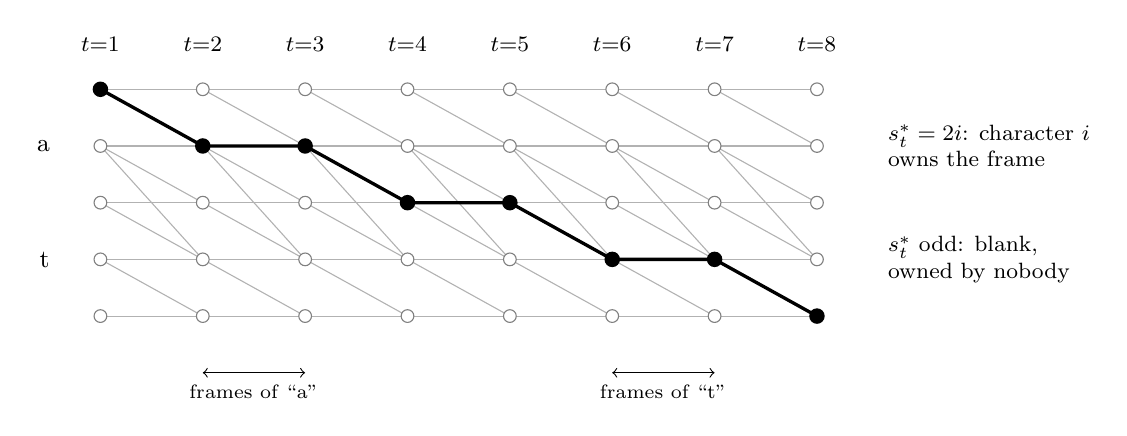
\begin{tikzpicture}[x={(1.3cm,0)},y={(0,-0.72cm)}]
\foreach \t in {1,...,7} {
  \foreach \s in {1,...,5} {\draw[gray!60] (\t,\s) -- (\t+1,\s);}
  \foreach \s in {1,...,4} {\draw[gray!60] (\t,\s) -- (\t+1,\s+1);}
  \draw[gray!60] (\t,2) -- (\t+1,4);
}
\foreach \t in {1,...,8} {\foreach \s in {1,...,5} {\fill[white,draw=gray] (\t,\s) circle (2.3pt);}}
\foreach \s/\l in {1/$\varnothing$,2/a,3/$\varnothing$,4/t,5/$\varnothing$} {\node[font=\small,anchor=east] at (0.6,\s) {\l};}
\foreach \t in {1,...,8} {\node[font=\footnotesize,anchor=south] at (\t,0.5) {$t{=}\t$};}
\draw[very thick] (1,1) -- (2,2) -- (3,2) -- (4,3) -- (5,3) -- (6,4) -- (7,4) -- (8,5);
\foreach \t/\s in {1/1,2/2,3/2,4/3,5/3,6/4,7/4,8/5} {\fill (\t,\s) circle (2.8pt);}
\draw[<->] (2,6.0) -- (3,6.0); \node[font=\scriptsize,anchor=north] at (2.5,6.05) {frames of ``a''};
\draw[<->] (6,6.0) -- (7,6.0); \node[font=\scriptsize,anchor=north] at (6.5,6.05) {frames of ``t''};
\node[font=\footnotesize,anchor=west,align=left] at (8.6,2) {$s^*_t=2i$: character $i$\\ owns the frame};
\node[font=\footnotesize,anchor=west,align=left] at (8.6,4) {$s^*_t$ odd: blank,\\ owned by nobody};
\end{tikzpicture}
\caption{Forced-alignment lattice for the transcript ``at'' with $T=8$ steps (cf.\ Figure~\ref{fig:rec-ctc}). The thick path is the Viterbi path of Equation~\ref{eq:sty-viterbi}; only the frames on the row of a letter belong to that letter, so the spans are narrow.}
\label{fig:sty-lattice}
\end{figure}

\begin{figure}[h]
\centering
\begin{tikzpicture}[x=0.82cm,y=0.82cm]
\newcommand{\dppoly}[1]{\draw[#1] (0,0) -- (0.8,0.3) -- (1.5,0.3) -- (2.2,1.2) -- (3.0,1.5) -- (3.8,1.45) -- (4.6,2.0) -- (5.4,1.9) -- (6.0,2.3);}
\dppoly{thick}
\foreach \p in {(0,0),(0.8,0.3),(1.5,0.3),(2.2,1.2),(3.0,1.5),(3.8,1.45),(4.6,2.0),(5.4,1.9),(6.0,2.3)} {\fill \p circle (1.8pt);}
\draw[dashed] (0,0) -- (6.0,2.3);
\draw[gray,dotted] (-0.107,0.280) -- (5.893,2.580);
\draw[gray,dotted] (0.107,-0.280) -- (6.107,2.020);
\draw[<->] (2.2,1.2) -- (2.32,0.889);
\node[font=\scriptsize,anchor=west] at (2.0,0.72) {$d_{\max}>\varepsilon$};
\node[font=\scriptsize,anchor=east] at (-0.15,0) {$a$};
\node[font=\scriptsize,anchor=west] at (6.1,2.3) {$b$};
\node[font=\scriptsize] at (2.2,1.55) {$p_k$};
\node[font=\scriptsize,anchor=north] at (3.0,-0.5) {(a) first split};
\begin{scope}[xshift=8.0cm]
\dppoly{gray}
\draw[very thick] (0,0) -- (1.5,0.3) -- (2.2,1.2) -- (6.0,2.3);
\foreach \p in {(0,0),(1.5,0.3),(2.2,1.2),(6.0,2.3)} {\fill \p circle (2.4pt);}
\node[font=\scriptsize,anchor=north] at (3.0,-0.5) {(b) simplified result};
\end{scope}
\end{tikzpicture}
\caption{Douglas--Peucker simplification (schematic, tolerance exaggerated). (a) The vertex $p_k$ with the largest distance $d_{\max}$ from the chord $ab$ lies outside the tolerance band (dotted) and splits the chain. (b) After recursion on both halves four of the original nine vertices remain.}
\label{fig:sty-dp}
\end{figure}

\begin{figure}[h]
\centering
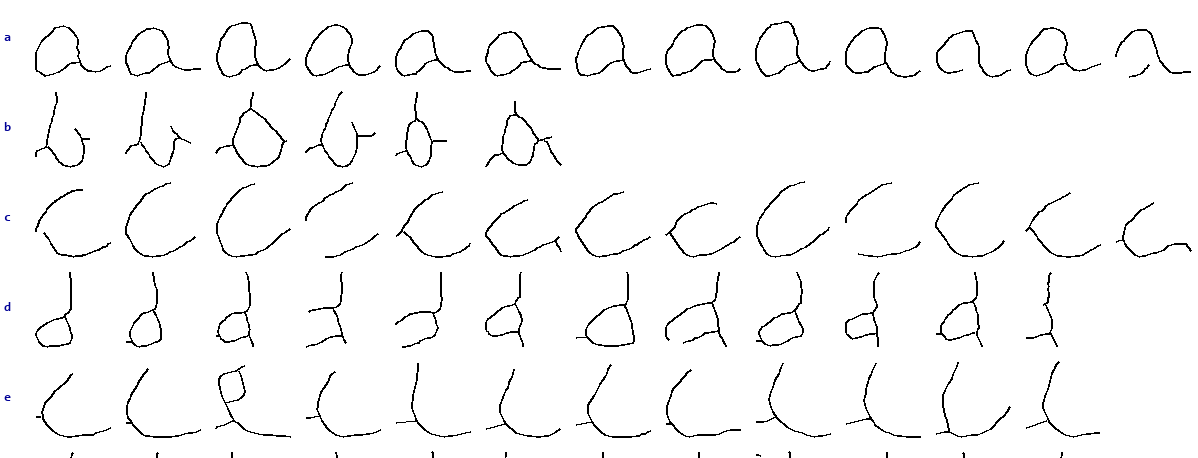
\includegraphics[width=\linewidth]{Figures/w3_glyphs153_ae.png}
\caption{Stored variants of the letters a, b, c, d and e of writer 153 (a strongly joined hand) in the glyph grid of the web interface; each row is one character with up to 12 variants. The short tails at the sides are remains of ligatures.}
\label{fig:sty-glyphs}
\end{figure}

\begin{figure}[h]
\centering
\figplaceholder{3.4cm}{One real line of a database writer and one personal line: grey crop, ink mask with rules removed and core band, Zhang--Suen skeleton, traced chains in colours with the territory cuts as vertical lines, and one extracted glyph in the normalised frame. Source: the functions of the profile builder applied to a crop of \texttt{Data/Datasets/IAMpages10} and one of \texttt{Software/CNN/NOGIT/dylan}.}
\caption{Stages of the style builder on real lines (placeholder).}
\label{fig:sty-stages}
\end{figure}

\begin{figure}[h]
\centering
\begin{tikzpicture}[x=1cm,y=1cm]
\newcommand{\hshape}[1]{\draw[#1] (0.1,0) -- (0.1,1.8); \draw[#1] (0.1,0.6) .. controls (0.3,1.0) and (0.7,1.0) .. (0.75,0.6) -- (0.75,0);}
\draw[gray] (-0.3,0) -- (4.3,0); \node[w3lab,anchor=east] at (-0.3,0) {baseline};
\draw[gray,dashed] (-0.3,1) -- (4.3,1); \node[w3lab,anchor=east] at (-0.3,1) {$y{=}1$};
\begin{scope}[xshift=0.2cm]\hshape{thick}\end{scope}
\begin{scope}[xshift=2.6cm,xslant=0.466]\hshape{thick}\end{scope}
\draw[w3arr] (1.2,0.9) -- (2.2,0.9);
\node[w3lab] at (1.7,1.15) {shear};
\draw[dotted] (2.7,0) -- (2.7,1.8);
\node[font=\scriptsize] at (2.0,-0.45) {(a) $X=\ell+x+y\tan\theta$};
\begin{scope}[xshift=6.3cm]
\draw[gray] (-0.3,0) -- (7.2,0);
\draw[fill=gray!10] (0,0) rectangle (2.3,1.4);
\draw[fill=gray!10] (2.3,0) rectangle (4.3,1.4);
\draw[thick] (0.5,0.1) rectangle (1.9,1.2);
\draw[thick] (2.55,0.1) rectangle (4.0,1.2);
\draw[<->] (0,-0.25) -- (2.3,-0.25); \node[w3lab,anchor=north] at (1.15,-0.25) {advance $a$};
\draw[<->] (0,1.6) -- (0.5,1.6); \node[w3lab,anchor=south] at (0.25,1.6) {$\ell$};
\draw[<->] (1.9,1.6) -- (2.55,1.6); \node[w3lab,anchor=south] at (2.3,1.6) {gap};
\draw[w3arr] (0,-0.9) -- (0.9,-0.9) node[midway,below,w3lab] {$P_x$};
\node[w3lab,anchor=west] at (4.4,0.7) {word gap $g\,x_{\mathrm{mm}}(0.85{+}0.3u)$};
\node[font=\scriptsize] at (3.2,-1.3) {(b) cells, ink boxes and guard};
\end{scope}
\end{tikzpicture}
\caption{Glyph placement. (a) A stored upright glyph is sheared by the writer's slant (Equation~\ref{eq:syn-place}). (b) Each glyph occupies a cell of its own advance $a$; the ink starts after the lead $\ell$, and the collision guard keeps a minimum clear gap between consecutive ink boxes.}
\label{fig:syn-layout}
\end{figure}

\begin{figure}[h]
\centering

\includegraphics[width=\linewidth]{Figures/w3_synth_150.png}\\[2pt]

\includegraphics[width=\linewidth]{Figures/w3_synth_153.png}
\caption{Synthesised line ``The gantry writes this sentence for the first time today'' for writer 150 (upper, printed hand; read back with three small errors) and writer 153 (lower, joined hand; read back as ``the garoby writes tttas senkence for tthe furst tuse today''), one seed and candidate each, rendered from the trajectory of an end-to-end run; the $N$ of that run was not recorded.}
\label{fig:syn-lines}
\end{figure}

\begin{figure}[h]
\centering
\begin{tikzpicture}[x=0.0225cm,y=0.0225cm]
\draw[fill=gray!8] (0,0) rectangle (204,262);
\draw[dashed] (5,5) rectangle (199,257);
\draw[thick] (5,5) rectangle (205,205);
\draw[thick,fill=gray!30] (15,40) rectangle (195,185);
\draw[w3arr] (5,5) -- (45,5) node[right,font=\scriptsize] {$X$};
\draw[w3arr] (5,5) -- (5,45) node[above,font=\scriptsize] {$Y$};
\fill (5,5) circle (3pt); \node[font=\scriptsize,anchor=north west] at (7,3) {machine $(0,0)$};
\fill (15,185) circle (3pt); \node[font=\scriptsize,anchor=south west] at (17,186) {$(X_{\mathrm{o}},Y_{\mathrm{o}})$};
\node[font=\scriptsize] at (105,110) {text block (illustrative)};
\draw[<->] (0,-18) -- (204,-18); \node[font=\scriptsize,anchor=north] at (102,-20) {204 mm switch-to-switch (X)};
\draw[<->] (-18,0) -- (-18,262); \node[font=\scriptsize,rotate=90,anchor=south] at (-20,131) {262 mm (Y)};
\node[font=\scriptsize,anchor=west,align=left] at (232,232) {dashed: driver usable area\\ $194\times252$ mm (5 mm edges)};
\node[font=\scriptsize,anchor=west,align=left] at (232,135) {solid: generator work area\\ $200\times200$ mm};
\end{tikzpicture}
\caption{Coordinate frames drawn to scale. The machine frame has its origin 5\,mm inside the minimum switches; the generator places the text block with its top-left corner at $(10,180)$\,mm inside a $200\times200$\,mm work area, and the driver clamps all targets to its calibrated usable area of $194\times252$\,mm. The extent of the text block is illustrative.}
\label{fig:gc-frames}
\end{figure}

\begin{table}[h]
\centering
\fontsize{9.5}{11.5}\selectfont
\begin{tabularx}{\linewidth}{|X|c|c|c|}
\hline
\textbf{Quantity (56-character sentence)} & \textbf{Writer 150} & \textbf{Writer 153} & \textbf{Writer 551} \\
\hline
Render size (pixels) & $3585\times225$ & $5508\times207$ & $7876\times277$ \\
\hline
Synthesis of one candidate (ms) & 11 & 13 & 16 \\
\hline
Rendering (ms) & 20 & 27 & 56 \\
\hline
Text recogniser (s) & 0.50 & 0.49 & 0.74 \\
\hline
Writer classifier incl. stroke normalisation (s) & 1.03 & 1.65 & 3.74 \\
\hline
Complete search, $N=14$, with repair attempts (s) & 23 & 37 & 137 \\
\hline
\end{tabularx}
\caption{Indicative cost of the search on the development laptop (single profiling run, unknown background load, jitter 0.5); times on the single-board computer were not recorded.}
\label{tab:syn-cost}
\end{table}

\subsection{Hardware information and timing measurements still to be supplied}

This part of the appendix supports Sections~\ref{sec:gantry} and~\ref{sec:system}.
Table~\ref{tab:gan-hw} lists the hardware items with the evidence in the project files, Figure~\ref{fig:gan-photo} is the placeholder for the photographs, and Table~\ref{tab:sys-timing} lists the stages of the timing chains.

\begin{table}[!htbp]
\centering
\fontsize{9.5}{11.5}\selectfont
\begin{tabularx}{\linewidth}{|p{2.6cm}|X|}
\hline
\textbf{Item} & \textbf{Evidence, and content to be supplied} \\
\hline
Computer & ODROID N2+ with 3.3\,V pins (Table~\ref{tab:gan-pins}). \\
\hline
Motors, drivers, transmission & Two motors with STEP/DIR driver modules; the program assumes 200 full steps per revolution, an A4988 at 1/16 microstepping and 40\,mm per revolution (2\,mm belt, 20-tooth pulley), and replaces the last by calibration. \textbf{[TO BE COMPLETED BY STUDENT: motor model, holding torque, rated current; driver model, current-limit setting, microstepping jumpers, minimum STEP pulse width; belt or screw type, pulley teeth, guides; whether any level shifter lies between the 3.3\,V pins and the drivers.]} \\
\hline
Travel & Measured switch-to-switch distances 204\,mm (X) and 262\,mm (Y). \textbf{[TO BE COMPLETED BY STUDENT: the calibrated steps per millimetre printed for both axes.]} \\
\hline
End-stops & Four switches, active-high at 3.3\,V, each with a pull-down of about 10\,k$\Omega$ (Figure~\ref{fig:gan-switch}). \textbf{[TO BE COMPLETED BY STUDENT: switch type and mounting.]} \\
\hline
Pen mechanism & One-direction gear motor whose cam toggles the pen every $90^\circ$, with a pen switch (high = up) (Section~\ref{sec:gan-pen}). \textbf{[TO BE COMPLETED BY STUDENT: how the motor is switched (transistor, flyback diode), supply voltage, pen model and holder, lift height.]} \\
\hline
Power supply (FU 4) & \textbf{[TO BE COMPLETED BY STUDENT: voltages and current ratings of the motor, computer and pen-motor supplies, grounding scheme, camera supply.]} The program comments state that the motors have no flyback diodes and share a ground return, which makes the switch inputs noisy (Section~\ref{sec:gan-stop}). \\
\hline
Camera (FU 1) & Generic USB video-class camera. \textbf{[TO BE COMPLETED BY STUDENT: model, resolution, mounting height, field of view, lamp.]} \\
\hline
\end{tabularx}
\caption{Hardware items: evidence in the project files and information still to be supplied.}
\label{tab:gan-hw}
\end{table}

\begin{figure}[!htbp]
\centering
\figplaceholder{2.4cm}{Photographs of the assembled gantry (axes, end-stops, pen holder with toggle motor, paper holder) and of the scanning rig with camera; CAD renderings and a wiring diagram with component values. To be supplied by the student.}
\caption{Photographs of the gantry and the scanning rig (placeholder).}
\label{fig:gan-photo}
\end{figure}

\begin{table}[!htbp]
\centering
\fontsize{9.5}{11.5}\selectfont
\begin{tabularx}{\linewidth}{|p{3.4cm}|X|}
\hline
\textbf{Stage} & \textbf{Known information and value to be supplied} \\
\hline
Capture & Framing by the user; five discarded frames without preview. \textbf{[TO BE COMPLETED BY STUDENT: time from pressing capture to the stored image.]} \\
\hline
Conditioning and segmentation & Whole page on the board. \textbf{[TO BE COMPLETED BY STUDENT: time per page on the board.]} \\
\hline
Recognition and writer classification & Two passes of about $4\times10^9$ multiply--accumulate operations per line. \textbf{[TO BE COMPLETED BY STUDENT: time per line on the board and total for the R4 test paragraph.]} \\
\hline
Synthesis & Returned in the server response; laptop values in Table~\ref{tab:syn-cost}. \textbf{[TO BE COMPLETED BY STUDENT: time on the board for the $N$ used in the demonstration.]} \\
\hline
G-code and preview & Milliseconds (not measured). \\
\hline
Gantry motion & Model 2.4 to 2.8\,s per character (Section~\ref{sec:gan-timing}). \textbf{[TO BE COMPLETED BY STUDENT: stopwatch time of a sentence of known length, from send to the final pen lift.]} \\
\hline
\end{tabularx}
\caption{Stages of the timing chains of the two modes and the measurements still missing.}
\label{tab:sys-timing}
\end{table}

\subsection{Design alternatives}

Tables~\ref{tab:sty-alt} and~\ref{tab:syn-alt} list the design alternatives of Sections~\ref{sec:styleprofile} and~\ref{sec:synthesis} with the reason for the chosen design.

\begin{table}[!htbp]
\centering
\fontsize{9.5}{11.5}\selectfont
\begin{tabularx}{\linewidth}{|p{3.0cm}|X|X|}
\hline
\textbf{Decision} & \textbf{Alternative} & \textbf{Reason for the chosen design} \\
\hline
Character boundaries & Fixed widths, projection minima, hand labelling. & Joined letters have no gaps and hand labelling of about 90 pages is impractical; the recogniser knows the text, so alignment is automatic. \\
\hline
Thin whole line, then cut & Thin each slice. & A slice edge creates a spurious spine stored as a bar. \\
\hline
Several variants per letter & One averaged letter. & Averaging blurs letters whose strokes are arranged differently; variants keep the natural variation, medoid and prototype remain options. \\
\hline
Prior as a filter & Import the median shape into every writer. & Importing would erase the writer; filtering keeps the shapes the writer's own. \\
\hline
Glyphs from scanned pages & Generator learned from on-line pen data. & No on-line data of the ten writers exist (47 to 138 usable lines each), and the pen path must be recovered from the image in any case (Section~\ref{sec:synthesis}). \\
\hline
\end{tabularx}
\caption{Design alternatives for the style extraction.}
\label{tab:sty-alt}
\end{table}

\begin{table}[!htbp]
\centering
\fontsize{9.5}{11.5}\selectfont
\begin{tabularx}{\linewidth}{|p{3.2cm}|X|}
\hline
\textbf{Alternative} & \textbf{Assessment} \\
\hline
Recurrent sequence generator with attention and mixture-density output \cite{graves2013} & Natural cursive, but needs on-line pen data (hundreds to thousands of lines per writer); only 47 to 138 scanned lines per writer exist. A from-scratch version trained on skeleton-derived strokes learned slant, roundness and connectedness but no legible letters. Rejected. \\
\hline
Adversarial or diffusion image generators \cite{kang2020,dai2024} & Low data need through pre-training, but the output is a raster: it needs vectorisation with the same thinning artefacts, size, slant and spacing cannot be controlled, and a trial took 35 to 45\,s (one line, laptop processor) to 2--3\,min against 3 to 8\,s for glyph synthesis. Rejected and parked. \\
\hline
Glyph assembly from one writer's sample \cite{haines2016} & Related approach; the present design adds the recogniser-aligned profile and the judge-driven search. \\
\hline
Glyph library with search (chosen) & Needs about nine pages per writer and no training; pen strokes are the native output; size, slant, joins and gap are explicit numbers; failures trace to one glyph; every glyph has a fallback. Weakness: cursive hands, whose joins are lost by cutting. \\
\hline
\end{tabularx}
\caption{Alternatives to the glyph-library synthesiser (timings are trial runs on a laptop without accelerator).}
\label{tab:syn-alt}
\end{table}

\subsection{Further figures and tables for Sections 3.8 to 3.10}

This part of the appendix supports Sections~\ref{sec:gcode} to~\ref{sec:system}.
Figure~\ref{fig:gc-excerpt} shows the start of a generated G-code program, Figure~\ref{fig:gc-vel} the velocity profiles of Equation~\ref{eq:gc-trap}, Table~\ref{tab:gan-pins} the pin assignment, Figure~\ref{fig:gan-switch} the switch input circuit and Table~\ref{tab:sys-modes} the chains of operations of the two online modes.

\begin{figure}[!htbp]
\begin{lstlisting}[basicstyle=\ttfamily\footnotesize,frame=none]
; Handwriting-Robot G-code -- author yeukita
; steps/mm  X=80.000  Y=80.000 (3200 microsteps/rev)
G21   ; millimetres
G90   ; absolute
G0 F2400                      <- travel feed, emitted once
G0 X10.059 Y179.271           <- travel to the first stroke
M3   ; pen DOWN (one 90deg pulse of the one-way gear motor)
G4 P0.350   ; wait for the 90deg rotation to finish
G1 F900                       <- draw feed
G1 X10.084 Y178.920           <- one line per vertex (0.35 mm apart)
...
M5   ; pen UP (one 90deg pulse of the one-way gear motor)
G4 P0.350
...                           <- next stroke; at the end: park, M2
\end{lstlisting}
\caption{Start of a generated program (test word of writer yeukita: 14 strokes, 239 draw moves, vertices 0.348\,mm apart on average); the arrows are annotations.}
\label{fig:gc-excerpt}
\end{figure}

\begin{figure}[!htbp]
\centering
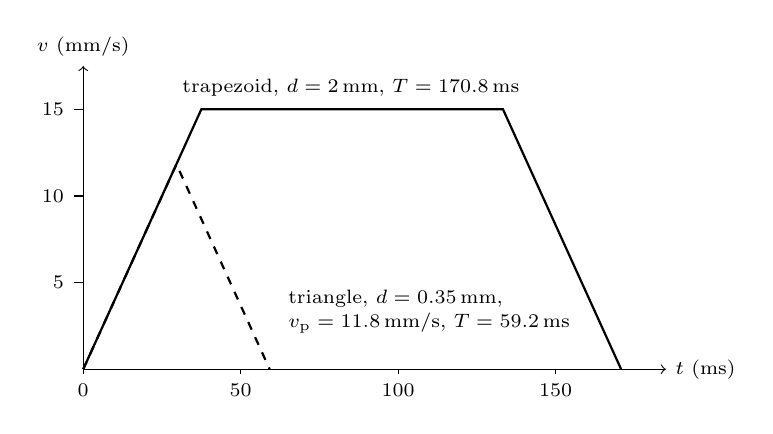
\begin{tikzpicture}[x=0.04cm,y=0.22cm]
\draw[->] (0,0) -- (185,0) node[right,font=\scriptsize] {$t$ (ms)};
\draw[->] (0,0) -- (0,17.5) node[above,font=\scriptsize] {$v$ (mm/s)};
\foreach \t in {0,50,100,150} {\draw (\t,0) -- (\t,-0.3) node[below,font=\scriptsize] {\t};}
\foreach \v in {5,10,15} {\draw (0,\v) -- (-3,\v) node[left,font=\scriptsize] {\v};}
\draw[thick] (0,0) -- (37.5,15) -- (133.3,15) -- (170.8,0);
\draw[thick,dashed] (0,0) -- (29.6,11.83) -- (59.2,0);
\node[font=\scriptsize,anchor=south] at (85,15.2) {trapezoid, $d=2$\,mm, $T=170.8$\,ms};
\node[font=\scriptsize,anchor=south west] at (62,3.0) {triangle, $d=0.35$\,mm,};
\node[font=\scriptsize,anchor=south west] at (62,1.5) {$v_{\mathrm p}=11.8$\,mm/s, $T=59.2$\,ms};
\end{tikzpicture}
\caption{Velocity profiles of Equation~\ref{eq:gc-trap} for $a=400$\,mm/s$^2$ and $v=15$\,mm/s: a 2\,mm move is trapezoidal (solid); the usual 0.35\,mm segment is triangular (dashed) and never reaches the cruise speed.}
\label{fig:gc-vel}
\end{figure}

\begin{table}[!htbp]
\centering
\fontsize{9.5}{11.5}\selectfont
\begin{tabularx}{\linewidth}{|X|c|c|c|c|}
\hline
\textbf{Function} & \textbf{Offset} & \textbf{Header pin} & \textbf{Direction} & \textbf{Initial level} \\
\hline
X motor DIR / STEP & 64 / 68 & 7 / 11 & output & high / low \\
\hline
Y motor DIR / STEP & 81 / 69 & 12 / 13 & output & high / low \\
\hline
X\_MIN / X\_MAX switch & 72 / 65 & 15 / 16 & input & --- \\
\hline
Y\_MIN / Y\_MAX switch & 66 / 67 & 18 / 22 & input & --- \\
\hline
Pen-position switch & 70 & 33 & input & --- \\
\hline
Pen motor drive & 71 & 35 & output & low \\
\hline
\end{tabularx}
\caption{Pin assignment of the gantry driver on \texttt{/dev/gpiochip0}, requested in one call; the header pin numbers are those of the program comments and were not checked against the board pinout.}
\label{tab:gan-pins}
\end{table}

\begin{figure}[!htbp]
\centering
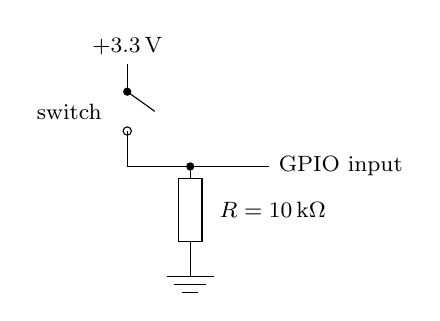
\begin{tikzpicture}[x=1cm,y=1cm,font=\footnotesize]
\draw (0,1.9) node[above] {$+3.3$\,V} -- (0,1.55);
\fill (0,1.55) circle (1.5pt); \draw (0,1.55) -- (0.35,1.3); \draw (0,1.05) circle (1.5pt); \draw (0,1.05) -- (0,0.6);
\node[anchor=east] at (-0.2,1.3) {switch};
\draw (0,0.6) -- (1.8,0.6) node[right] {GPIO input};
\fill (0.8,0.6) circle (1.5pt);
\draw (0.8,0.6) -- (0.8,0.45); \draw[fill=white] (0.65,0.45) rectangle (0.95,-0.35); \draw (0.8,-0.35) -- (0.8,-0.8);
\node[anchor=west] at (1.05,0.05) {$R=10$\,k$\Omega$};
\draw (0.5,-0.8) -- (1.1,-0.8); \draw (0.6,-0.9) -- (1.0,-0.9); \draw (0.7,-1.0) -- (0.9,-1.0);
\end{tikzpicture}
\caption{Switch input circuit as documented in the program comments; the closing current is $3.3\,\mathrm{V}/10\,\mathrm{k}\Omega=0.33$\,mA. The origin of the 3.3\,V (header pin) is inferred and \textbf{[TO BE CONFIRMED BY STUDENT]}.}
\label{fig:gan-switch}
\end{figure}

\begin{table}[!htbp]
\centering
\fontsize{9.5}{11.5}\selectfont
\begin{tabularx}{\linewidth}{|p{2.1cm}|p{2.1cm}|X|}
\hline
\textbf{Mode} & \textbf{Page} & \textbf{Chain of operations} \\
\hline
Classification & Read & Capture (live preview) or upload $\rightarrow$ conditioning and line segmentation $\rightarrow$ per line the text recogniser and the ink-based writer classifier $\rightarrow$ mean writer probabilities $\rightarrow$ text, writer, confidence and number of lines; with expected text and writer typed, also the character accuracy and a match mark. \\
\hline
Reproduction & Write & Calibrate once per session $\rightarrow$ text, writer and $N$ $\rightarrow$ best-of-$N$ synthesis $\rightarrow$ G-code, preview, read-back text and accuracy, pen pulses and synthesis time $\rightarrow$ ``send to gantry''. An uploaded G-code file uses the same preview and send path. \\
\hline
Training & (none) & Offline programs: segmentation of photographs, training of the networks and the profile builder (Section~\ref{sec:styleprofile}); the ten writers are pre-built files and the interface has no training function. \\
\hline
\end{tabularx}
\caption{Mapping of the proposal's modes to the web interface. A third page shows model architectures, sizes and stored accuracies, and for each writer sample crops and the glyph grid.}
\label{tab:sys-modes}
\end{table}

\subsection{Style calibration of the synthesiser}

Section~\ref{sec:syn-cal} describes the calibration; its three fixed-point iterations are, with ``ref'' the stored real-line value and ``got'' the value measured on the probe,
\begin{equation}
\Delta_\sigma\leftarrow\Delta_\sigma+\tan\theta_{\mathrm{ref}}-\tan\theta_{\mathrm{got}},\quad K_A\leftarrow\operatorname{clip}\Bigl(K_A\frac{A_{\mathrm{ref}}-1}{A_{\mathrm{got}}-1},0.5,1.6\Bigr),\quad K_D\leftarrow\operatorname{clip}\Bigl(K_D\frac{D_{\mathrm{ref}}}{D_{\mathrm{got}}},0.5,1.6\Bigr),
\label{eq:syn-cal}
\end{equation}
applied as $y\leftarrow1+(y-1)K_A$ for $y>1$ and $y\leftarrow yK_D$ for $y<0$ on the writer's own glyphs; $\Delta_\sigma$ is added to the shear coefficient of Equation~\ref{eq:syn-global}.
